%!TEX root = thesis.tex

\chapter{Introduction}

Operating a robot and developing high level control code for it is a cumbersome task. Very often various groups of developers are working simultaneously on different parts of the software. But in most cases there is only one device that can be used for testing and so only one can run his/her code at a time. The others have to wait until they get access to the robot. Moreover, tests on real robots always come with a high level of risk. Incorrect algorithms can lead very fast to damages on robot components or their environment and entail costly repairs. In the worst case even people can get hurt by uncontrolled robot motions.

The solution to those problems is the usage of a simulator that mimics the robot components and their behavior as accurate as possible. It has to provide the same control interface so that each part of the software can get tested on the simulator before it gets utilized on the real robot. Those considerations motivated the first part of this thesis -- the realistic replication of the IIS-Lab robot setup on a suitable simulation platform. This involves the creation of an exact model of the robot setup, containing the various robot components and their environment. The necessary steps are explained in Chapter~\ref{chap:simulation}.

The second part of the thesis is about motion planning. Moving the robot hand cannot follow any arbitrary trajectory towards a target pose. During that motion it might collide with itself or any other obstacle within it's environment. That means those trajectories have to be planned carefully to avoid accidental collisions and to generate smooth and well controlled robot motions. This also involves to create and maintain an internal representation of the robot and it's environment, a step that is common to the simulation part of the thesis. Chapter 3 shows the configuration and integration of the motion planning framework MoveIt into the IIS-Lab robot setup along with some usage examples.

Chapter 4 focuses on MoveIt's grasping functionality. It shows, how a reference `Pick and Place' task can be planned with the planning tools  and executed on the simulator and the real robot as well.

In Chapter 5, some test results will be presented, analyzing the quality of the various planning algorithms and approaches.

\section{IIS-Lab Robot Setup}
\begin{figure}[ht]
	\centering
  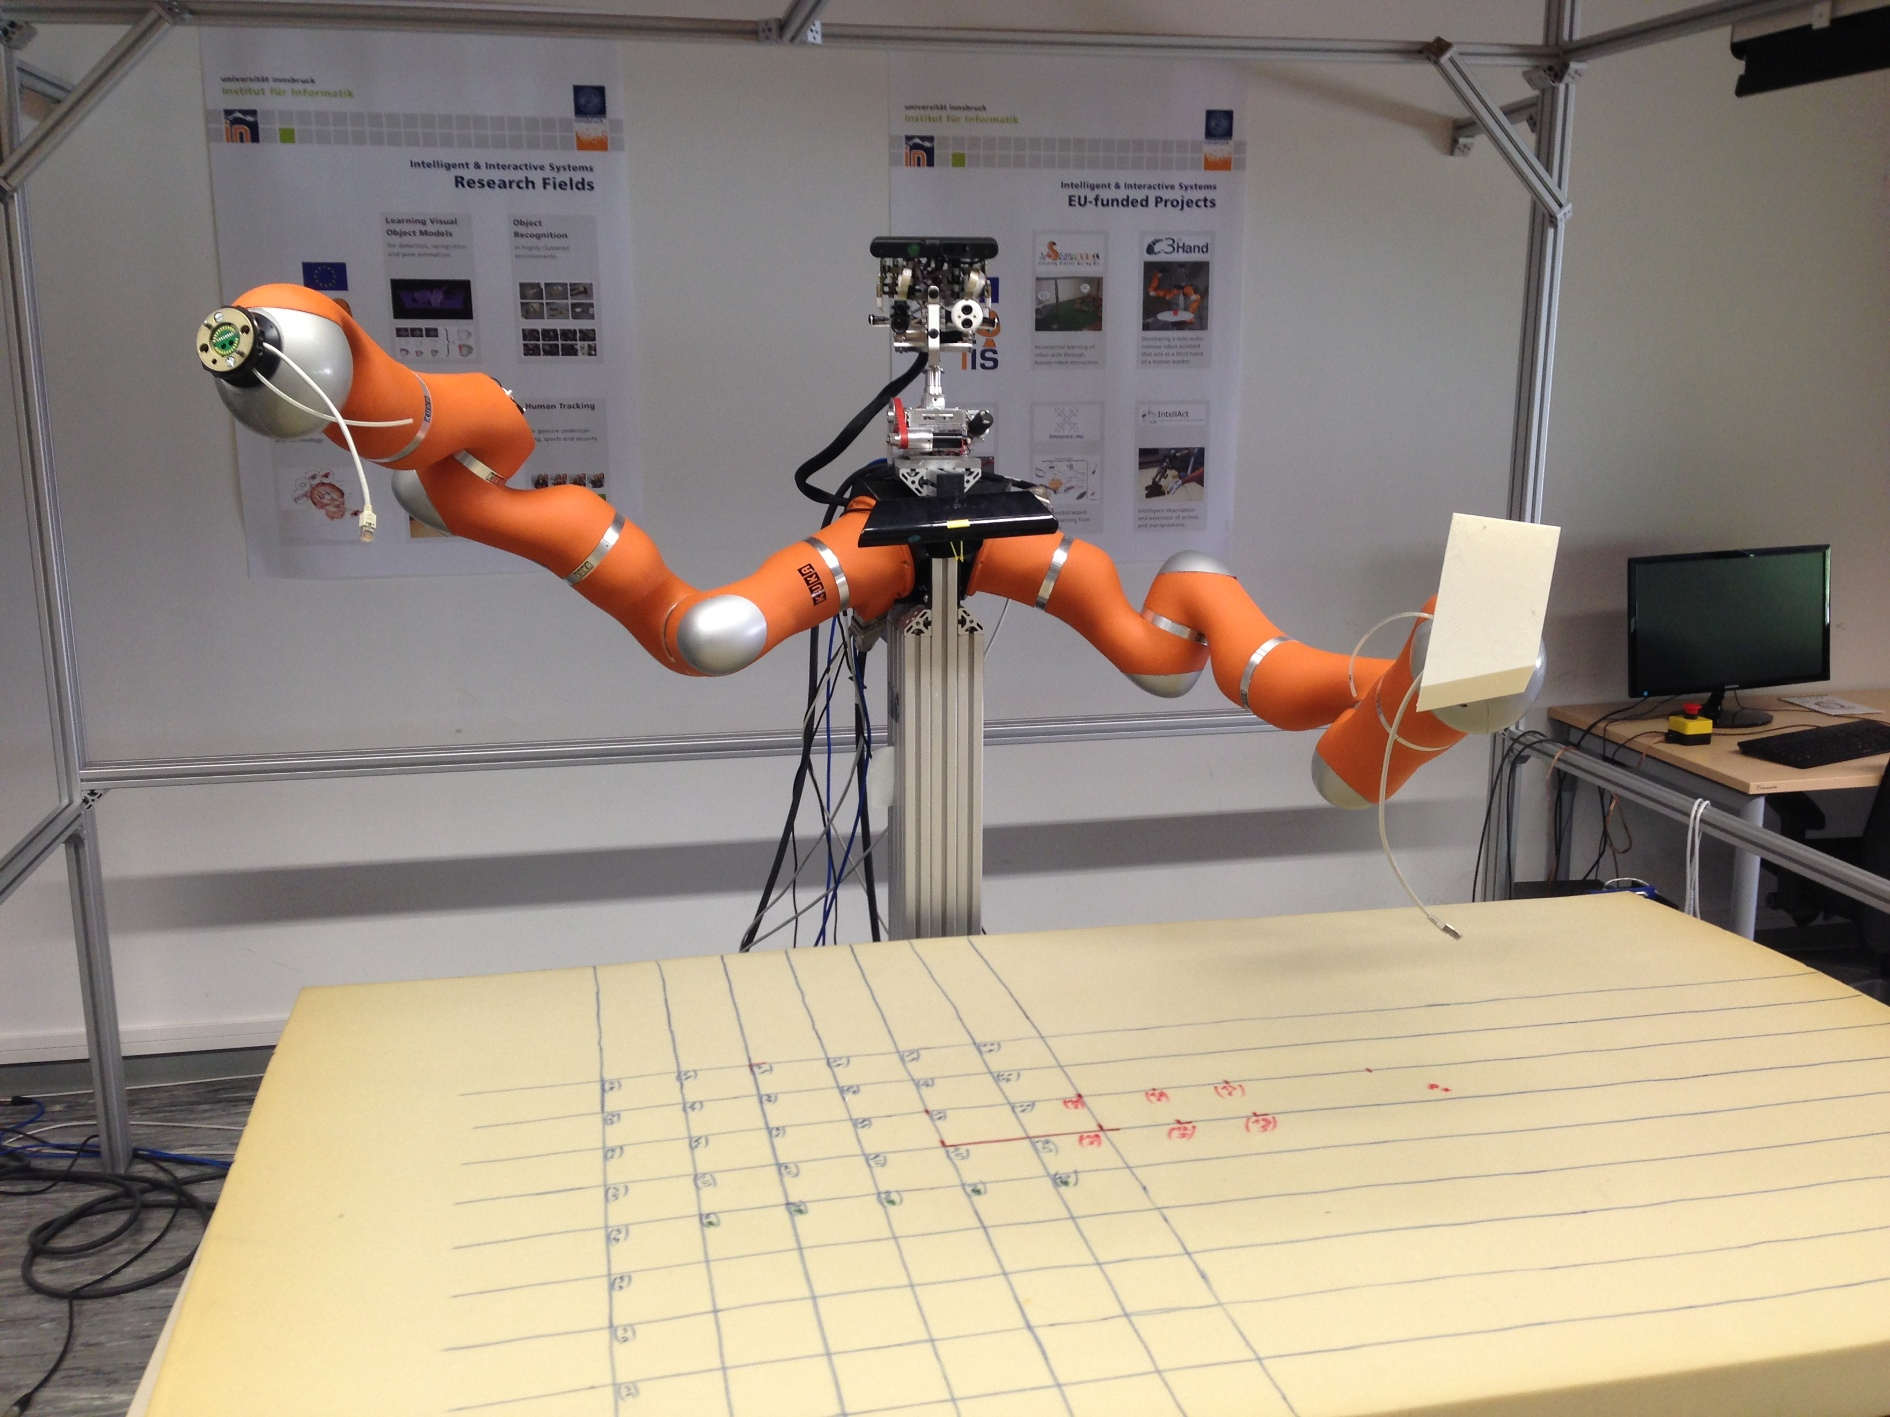
\includegraphics[width=0.75\textwidth]{images/robot_setup.jpg}
	\caption{Current setup in the IIS-Lab TODO: provide more recent image}
	\label{fig:fig1}
\end{figure}

The robot setting, that was considered in this thesis can be seen in Figure \ref{fig:fig1}
The main part of the robot setup in the IIS-Lab consists of an aluminium torso with two mounted KUKA light weight robot arms. Those arms have 7 degrees of freedom (DOF) each one can carry up to 7kg of payload. Additionally a Schunk SDH gripper can be mounted on each arm.

\begin{itemize}
	\item \textbf{KUKA LWR 4+ arm}\\
		Description of the arm(7 DOF, max. 7kg payload, 16kg weight, very flexible,...
	\item \textbf{Schunk SDH gripper}\\
		Description of the gripper(3-finger-gripper, different grasp types, as powerful as human hand, very sensitive)
	\item \textbf{Kinect camera}\\
		Description of Kinect(RGB camera, Depth sensor, 3d data under any light conditions)
\end{itemize}


\section{The Robot Operating System(ROS)}
As the control of the robot components is based on ROS, a brief introduction shall be given here. As stated in \cite{quigley2009}, ROS is not an operating system in the classical sense. It can be seen as a communication layer, providing various mechanisms for inter process communication. A ROS system consists of a number of nodes. Each node is an independent computation unit and runs in it's own process, adding some clearly defined functionality to the overall system. For example one node can be responsible for planning, another one for perception or controlling the hardware. Nodes communicate with each other by passing messages, using the ROS communication infrastructure. Messages are strictly typed data structures that can be defined in a special message composition language. They can be composed of primitive types like Float, Integer or Strings and also of other message types. That makes it possible to define custom messages for each use case. Messages can be published to topics. A topic can be seen as some kind of address, consisting of a string. Topics can be organized in namespaces. If two instances provide the same interface, each one can be operated in it's own namespace. This is important, as for example the simulator should provide exactly the same interface as the real robot. Without namespaces it would not be possible to operate the simulator and the real robot in parallel. So Each node can publish and also subscribe to a number of topics. It is also possible that more than one node publishes to the same topic. The organization of the nodes of a system can be visualized as a graph.

A node can also advertise a service. This is a special type of topic that allows a synchronized message exchange. In contrast to topics, a service with a given name can only be offered by one node. The service message is composed of a request and a response part. When a node sends a service request to another node it will block, until the advertising node has handled the request and delivers a response. The nodes that make up a ROS system can be located on different machines. One machine has to be the dedicated master that runs the roscore. Other machines can connect to the master via network. ROS also provides a centralized parameter server that can be used to store configuration data for the various nodes. A system usually consists of a large number of nodes that have to be configured and started. This can be done in launch files. Those are simple textfiles, holding startup information and configuration details for one or more nodes in an XML syntax. Using the roslaunch command, a set of nodes can be configured and launched at once. It is important to understand this terminology because especially the terms node, topic and message are heavily used throughout this thesis. A more detailed documentation can be found on the ROS website.

\section{Project Targets}
Both objectives

	\begin{itemize}
	
		\item \textbf{Simulation}\\
			Realistic replication of the robot setup on a suitable simulation platform
			Generation of realistic sensor data
			Visualization of collisions
			Implementation of a ROS interface, corresponding to that one of the real robot
		\item \textbf{Motion Planning}\\
			Configuration and integration of a motion planning framework
			Implementation of a benchmark pick and place task, executable on simulator and
			real robot
			Provide an easy to use interface to the planner
			Analyse the quality of the various planning algorithms
			
	\end{itemize}